%\documentclass[draft]{beamer}
%\documentclass[handout]{beamer}
\documentclass{beamer}

% This file is a solution template for:

% - Giving a talk on some subject.
% - The talk is between 15min and 45min long.
% - Style is ornate.



% Copyright 2004 by Till Tantau <tantau@users.sourceforge.net>.
%
% In principle, this file can be redistributed and/or modified under
% the terms of the GNU Public License, version 2.
%
% However, this file is supposed to be a template to be modified
% for your own needs. For this reason, if you use this file as a
% template and not specifically distribute it as part of a another
% package/program, I grant the extra permission to freely copy and
% modify this file as you see fit and even to delete this copyright
% notice. 


\mode<presentation>
{
  %\usetheme[compress]{Berlin}  
  %\usetheme{Berkeley}
  %\usecolortheme{sidebartab}
  \usetheme{Mainz}
  \setbeamercovered{dynamic}
  % or whatever (possibly just delete it)
  \usefonttheme{professionalfonts}
  \setbeamertemplate{navigation symbols}{}
  \setbeamertemplate{footline}[frame number]
}


%****************************************************************************************************
% PACCHETTI
%****************************************************************************************************
% Tema principale
%\usetheme{Mainz}

%\usepackage{fontspec}
%\usepackage[libertine={Ligatures=TeX,RawFeature=+onum},biolinum={Ligatures=TeX,RawFeature=+onum}]{libertineotf}

\usepackage[biolinum,sfdefault]{libertine}
\usepackage{eulervm}

\usepackage[italian]{babel}

\usepackage[T1]{fontenc}
\usepackage[utf8]{inputenc}

%\usepackage{beamerfoils}
%\usepackage{array}
%\usepackage{mathrsfs}
\usepackage{booktabs}
\usepackage{color}
\usepackage{colortbl}    
\usepackage[version=3]{mhchem} 
%\usepackage{gensymb}
\usepackage{tabularx}
%\usepackage{cancel}
\usepackage[labelformat=empty,labelsep=none,skip=1pt]{caption}
\usepackage[per-mode=symbol]{siunitx}
\usepackage{relsize,xspace}
\usepackage{bm}
\usepackage{pgfpages}

\usepackage{tikz}
\usetikzlibrary{shapes,arrows,shadows,mindmap,trees,calc}

\usepackage{lipsum}

%****************************************************************************************************

%\setbeamercovered{dynamic}

\def\arrowd{
  (10.75:1.1) -- (6.5:1) arc (6.25:120:1) [rounded corners=0.5] --
  (120:0.9) [rounded corners=1] -- (130:1.1) [rounded corners=0.5] --
  (120:1.3) [sharp corners] -- (120:1.2) arc (120:5.25:1.2)
  [rounded corners=1] -- (10.75:1.1) -- (6.5:1) -- cycle
}

\tikzset{
  ashadow/.style={opacity=.25, shadow xshift=0.07, shadow yshift=-0.07},
}


%****************************************************************************************************
% COLORI e STILI di TESTO
\definecolor{greendark}{RGB}{0,178,140}
\definecolor{bluegreen}{cmyk}{0.9,0.0,0.35,0.2}
\definecolor{darkblue}{rgb}{0.2,0.2,0.65}
\definecolor{themecolor}{rgb}{0.137,0.466,0.741} % blue


%\newcommand{\cit}{\scriptsize\color{bluegreen}}             % citazioni
\newcommand{\cit}{\scriptsize\color{themecolor!80!green}}             % citazioni
\newcommand{\tbtit}{\bf\color{themecolor!75!black}} % titoli nelle tabelle
\newcommand{\ev}{\color{themecolor}\bf}
%\renewcommand{\CancelColor}{\color{red}}
%****************************************************************************************************


%****************************************************************************************************
% TABELLE
\newcolumntype{C}[1]{>{\centering\let\newline\\\arraybackslash\hspace{0pt}}m{#1}}
\setlength{\aboverulesep}{0pt}
\setlength{\belowrulesep}{0pt}
\setlength{\extrarowheight}{.75ex}
\arrayrulecolor{themecolor!75!black}

\newcommand{\tabitem}{~~\llap{\textbullet}~~}
%****************************************************************************************************


%****************************************************************************************************
% FRECCE
\tikzset{bluearrow/.style={draw=themecolor,fill=themecolor,single arrow,drop shadow=%
                           {shadow xshift=.3ex,shadow yshift=-.3ex,color=themecolor!60!black},
                           minimum height=3.5ex,minimum width=0.1ex,single arrow head extend=0.5ex,
                           single arrow tip angle=70}}

\newcommand{\arrowup}{\tikz[baseline=-0.5ex]{\node[bluearrow,rotate=90]{};}}
\newcommand{\arrowdown}{\tikz[baseline=-0.5ex]{\node[bluearrow,rotate=-90]{};}}
\newcommand{\arrowright}{\tikz[baseline=-0.5ex]{\node[bluearrow]{};}}
\newcommand{\arrowleft}{\tikz[baseline=-0.5ex]{\node[bluearrow,rotate=180]{};}}
%****************************************************************************************************


% COMANDI PERSONALI
\newcommand{\gete}{\ce{GeTe}\xspace}

% Path per le immagini
\graphicspath{{Immagini/}{../Thesis/Immagini/Plots/}{../THESIS/Immagini/}{../THESIS/Immagini/Plots/}{../THESIS/Immagini/bulk_figures/}}



%\setbeameroption{show notes on second screen}
\setbeameroption{show notes}

%%% Layout di 4 pagine per foglio
%\pgfpagesuselayout{4 on 1}[a4paper,border shrink=5mm,landscape]


\title[] % (optional, use only with long paper titles)
{Simulazioni atomistiche del processo di cristallizzazione in nanofili per memorie a cambiamento di fase}

%\subtitle
%{Molecular dynamics simulations in microcanonical ensemble} % (optional)

\author[] % (optional, use only with lots of authors)
{Edoardo Baldi\\\medskip {\small\emph{Relatore:} Prof.~Marco~Bernasconi}}
% - Use the \inst{?} command only if the authors have different
%   affiliation.
\institute[]{Università di Milano--Bicocca --- Dipartimento di Fisica}

\date[] % (optional)
{{\small Sessione di Laurea Magistrale del} \\[3pt] 23 marzo 2015}

%\subject{Molecular Dynamics}
% This is only inserted into the PDF information catalog. Can be left
% out. 

% If you have a file called "university-logo-filename.xxx", where xxx
% is a graphic format that can be processed by latex or pdflatex,
% resp., then you can add a logo as follows:

%\pgfdeclareimage[height=0.5cm]{university-logo}{Logo_Green}
%\logo{\pgfuseimage{university-logo}}


% If you wish to uncover everything in a step-wise fashion, uncomment
% the following command: 

%\beamerdefaultoverlayspecification{<+->}


\begin{document}

{%
\setbeamertemplate{footline}{} % suppress number in titlepage
\begin{frame}
  \titlepage
\end{frame}
}

\addtocounter{framenumber}{-1} % resent frame counter

%\begin{frame}{Outline}
%  \tableofcontents
  % You might wish to add the option [pausesections]
%\end{frame}


\section{Introduzione}



%\subsection{Materiali e memorie a cambiamento di fase}

\begin{frame}{Materiali a cambiamento di fase per memorie ottiche ed elettroniche}
\begin{minipage}{1.0\textwidth}
  \begin{minipage}[b]{0.53\linewidth}
  Memorie ottiche: {\ev DVD--RW,\\ Blu--ray Disc}
  \end{minipage}
\hfill
  \begin{minipage}[b]{0.43\linewidth}\centering
  \includegraphics[angle=0, width=0.4\textwidth]{DVD}
  \end{minipage}
\end{minipage}
\begin{minipage}{1.0\textwidth}
  \begin{minipage}[b]{0.53\linewidth}
  Memorie elettroniche non volatili:\hfill\\ {\ev memorie a cambiamento di fase} (PCM)
  \end{minipage}
\hfill
  \begin{minipage}[b]{0.43\linewidth}\centering
  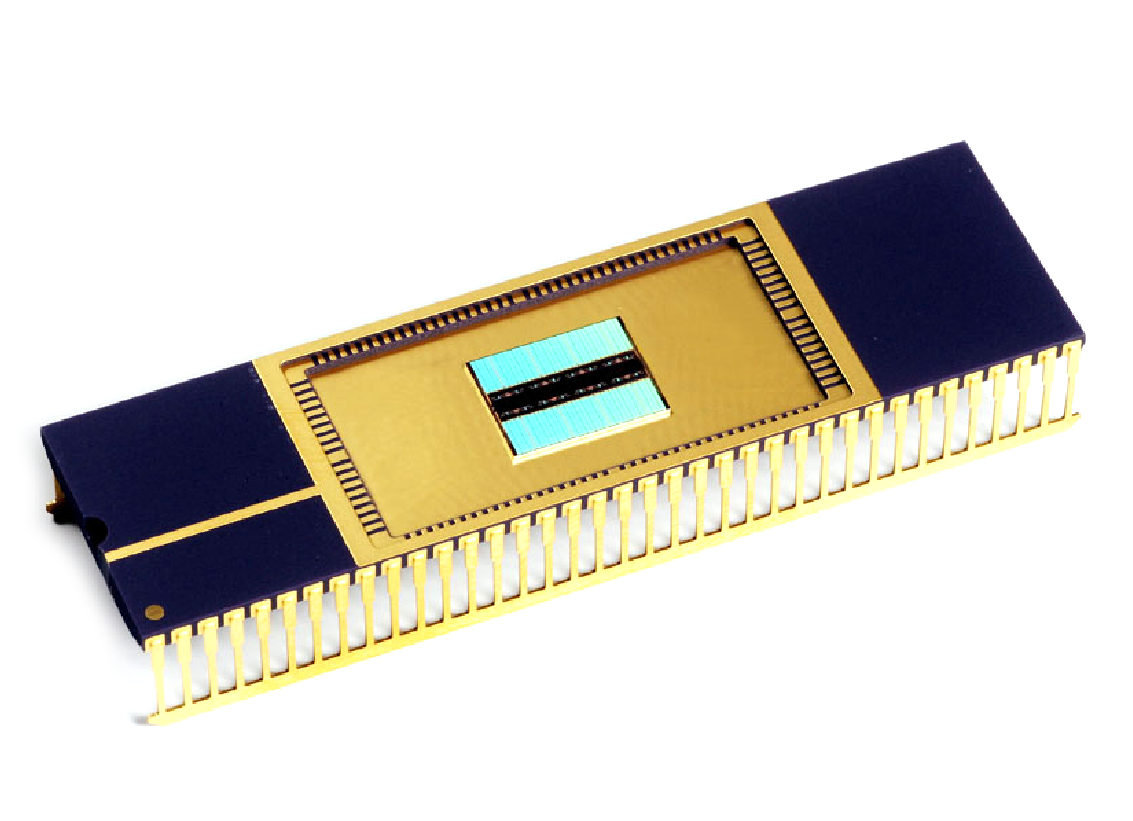
\includegraphics[angle=0, width=0.4\textwidth]{PCM}\\
  \end{minipage}
\end{minipage}
\vspace{1cm}\\
Leghe di calcogenuri: {\ev \gete}, \textcolor{themecolor}{\textbf{\ce{Ge2Sb2Te5} (GST)}}\\[6pt]
%\vspace{0.5cm}
\onslide<2->{
Rapida e reversibile transizione tra cristallo e amorfo ($\sim\SI{50}{ns}$)
}
\end{frame}
\note{%
I Materiali a Cambiamento di Fase sono di grande interesse tecnologico nella realizzazione di memorie non volatili ottiche, utilizzate in supporti come DVD e Blu--Ray, e memorie elettroniche di nuova concezione chiamate Memorie a Cambiamento di Fase.\\
Per le le memorie elettroniche, i materiali più utilizzati sono alcune leghe di calcogenuri basate su tellurio, come il germanio-tellurio o il germanio 2 antimonio 2 tellurio 5 o GST, il quale è attualmente impiegato come materiale attivo nelle PCM.\\
Tutti questi materiali mostrano una veloce e reversibile transizione tra la fase amorfa e la fase cristallina, che dura qualche decina di nanosecondi.
}


\begin{frame}{Materiali a cambiamento di fase}
\begin{table}
\begin{center}
\begin{tabular}{lcl}
Due stati della memoria & \arrowright & bit ``0'' o ``1''\\
\end{tabular}
\vspace{.5cm}\\
%\onslide<2->{
Grande differenza nelle proprietà tra le due fasi \\
%\vspace{1cm}
\begin{tabular}{ccc}
Fase cristallina & {\scriptsize $\arrowright$} & metallica \\
\end{tabular}
\quad
\begin{tabular}{ccc}
Fase amorfa & {\scriptsize $\arrowright$} & isolante\\
\end{tabular}
%}
\vspace{3ex}\\
%\onslide<3->{
\begin{tabular}{lcl}
Variazione di resistività di 3 ordini di grandezza & {\tiny $\arrowright$} & PCM\\
Differenza della riflettività del 30\% & {\tiny $\arrowright$} & memorie ottiche\\
\end{tabular}
\vspace{0.5cm}\\
La transizione è indotta per riscaldamento (impulsi laser/corrente)
%}
\end{center}
\end{table}
\end{frame}
\note{%
I due stati del sistema, ossia cristallo e amorfo, possono essere associati ai due stati della memoria (bit zero e bit uno). Questo è possibile grazie al fatto che questi materiali mostrano una grande differenza nelle proprietà delle due fase; in particolare, possiamo dire che il cristallo ha un comportamento metallico, mentre l'amorfo è isolante.\\
Una variazione di resistività di tre ordini di grandezza è alla base del funzionamento delle PCM, mentre un la variazione di riflettività (circa il 30\%) è sfruttata nelle memorie ottiche. In entrambi questi dispositivi, la transizione è indotta per riscaldamento, utilizzando impulsi di corrente nelle PCM e impulsi laser nei dispositivi ottici.
}


\begin{frame}{Cella PCM}
\begin{columns}
 \begin{column}{0.5\textwidth}
  \begin{itemize}
   \item {\ev Regione attiva}: piccola porzione del film di materiale che subisce la transizione
   \item Transizione indotta per effetto Joule
  \end{itemize}
 \end{column}
 \begin{column}{0.5\textwidth}
   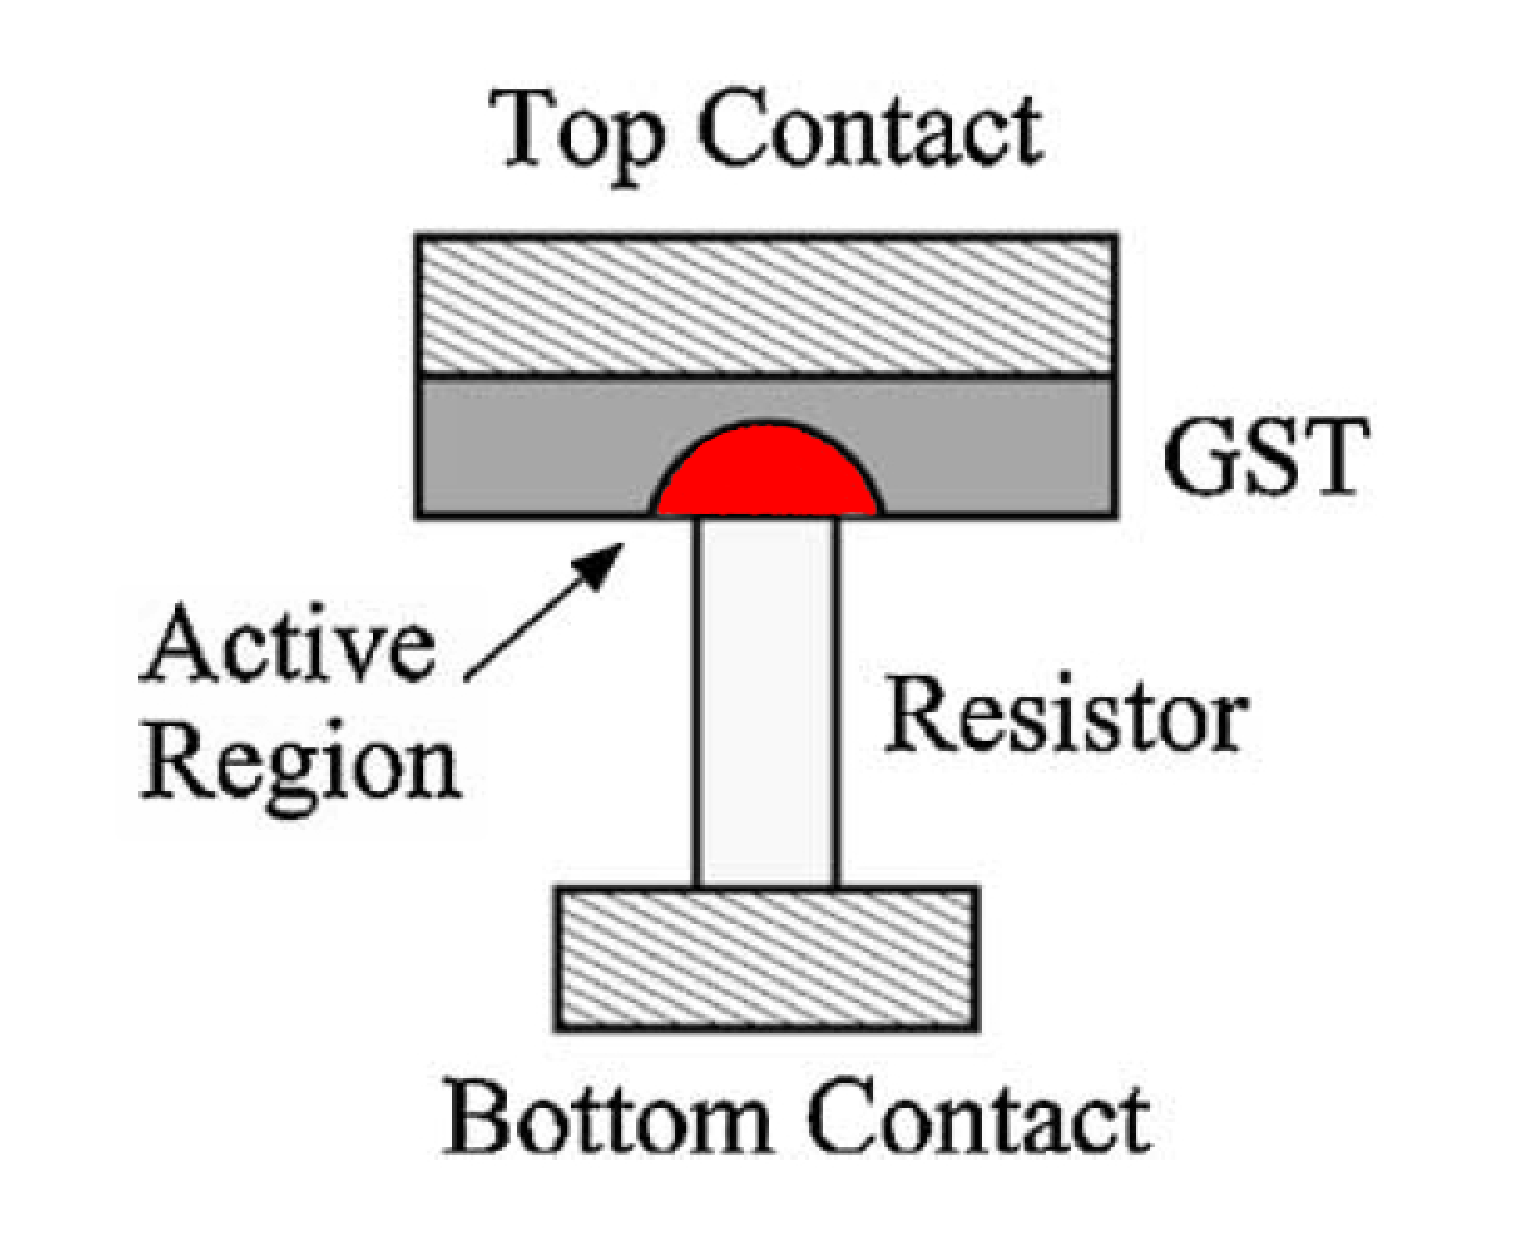
\includegraphics[scale=0.2]{PCMschem}
  %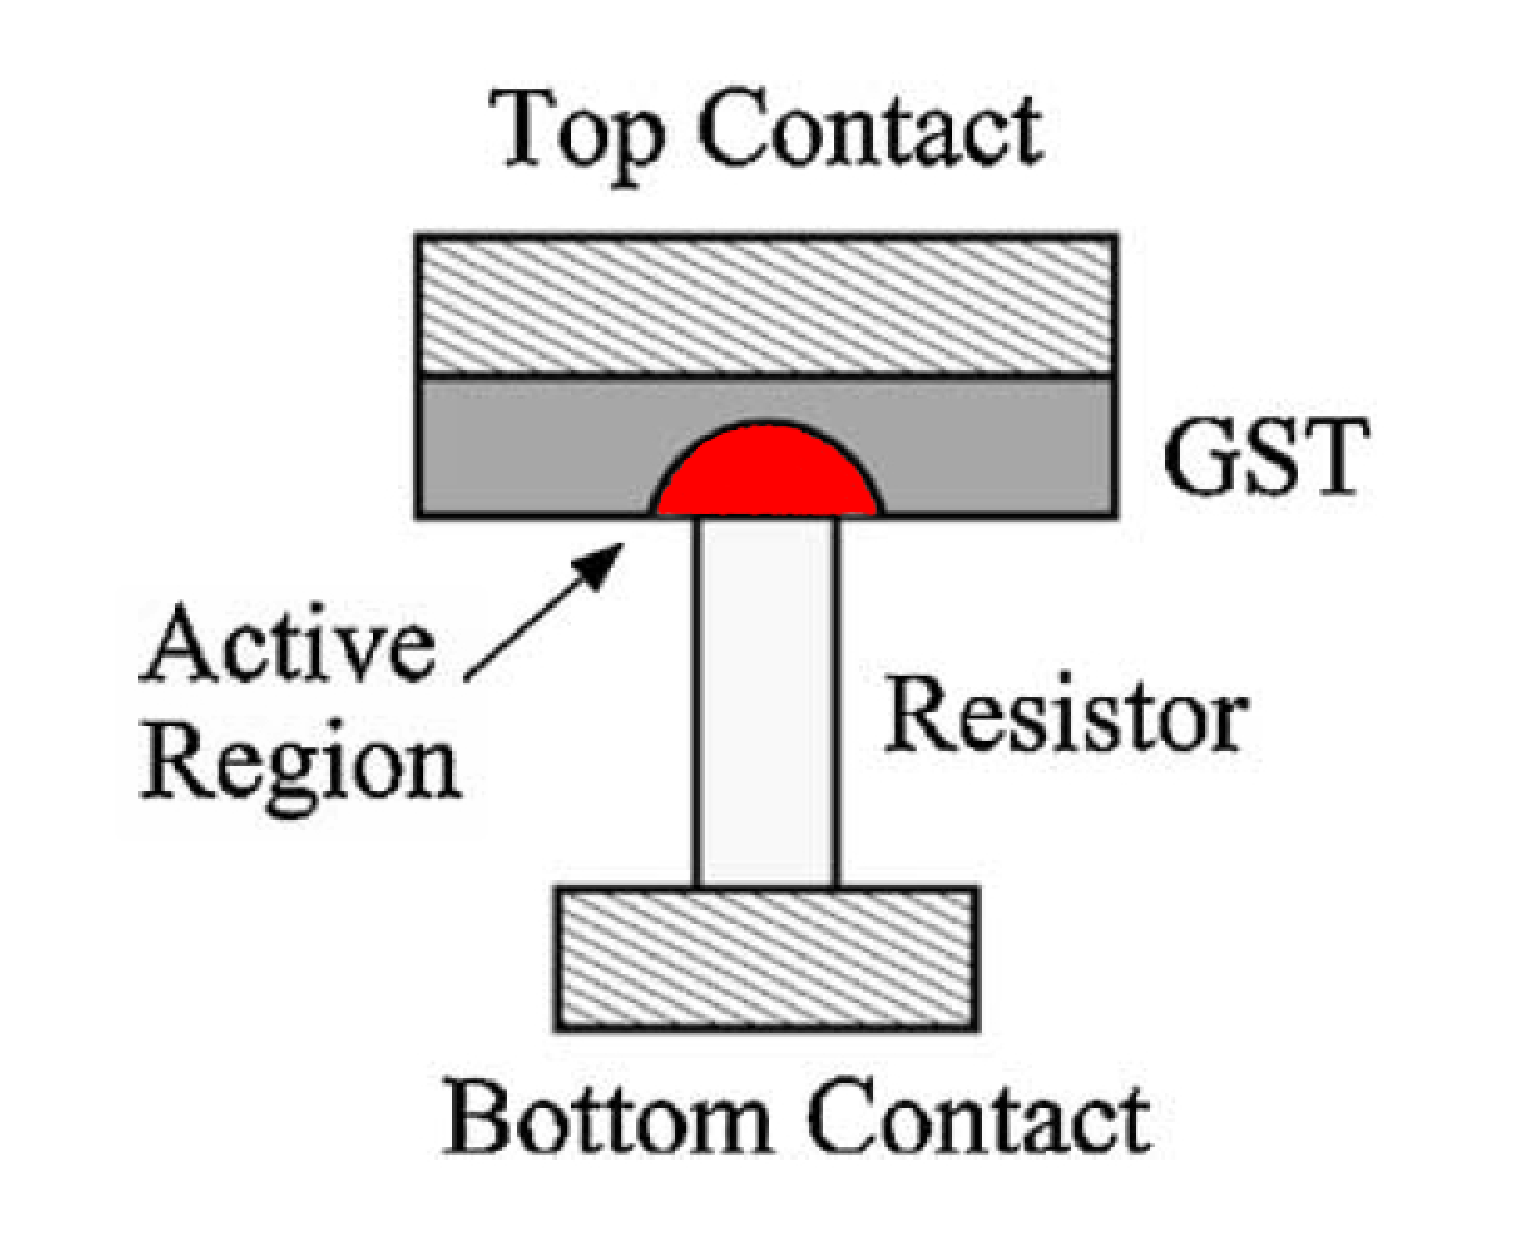
\includegraphics[width=0.5\textwidth]{PCMschem}
 \end{column}
\end{columns}
\end{frame}
\note{%
Una cella PCM è formata da un film di materiale a cambiamento di fase, posto tra un contatto metallico e un resistore. La regione attiva della cella è soltanto una porzione di materiale e la transizione avviene per riscaldamento dovuto all'effetto Joule.
}


\begin{frame}{Caratteristica I--V di una cella PCM}
\begin{columns}
 \begin{column}{0.5\textwidth}
  \begin{itemize}
    \item<2> \emph{Lettura}: eseguita a bassa tensione ($V < V\ped{th}$)
    \item<3-> Processi di \emph{set/reset}: tensione applicata maggiore del valore $V\ped{th}$)
    \begin{itemize}
      \item<3-> \emph{Reset}: elevata intensità di corrente e impulso breve \\
		\ev{cristallo} $\rightarrow$ \ev{amorfo}
      \item<4-> \emph{Set}: bassa intensità e impulso più lungo \\
		\ev{amorfo} $\rightarrow$ \ev{cristallo}
    \end{itemize}
   \end{itemize}
 \end{column}
  \begin{column}{0.5\textwidth}
   \includegraphics<1>[angle=0, width=1.0\textwidth]{IV1}
   \includegraphics<2>[angle=0, width=1.0\textwidth]{IVr}
   \includegraphics<3>[angle=0, width=1.0\textwidth]{IVres}
   \includegraphics<4>[angle=0, width=1.0\textwidth]{IVs}
  \end{column}
\end{columns}
\end{frame}
\note{%
La programmazione di una cella PCM è possibile grazie alla particolare caratteristica corrente--tensione del materiale attivo. L'immagine rappresenta una tipica curva corrente--tensione per un materiale a cambiamento di fase. Si noti come la fase cristallina ha un comportamento ohmico, mentre la fase amorfa manifesta un elevata resistività sino ad un valore di soglia, indicato con Vth. Al di sopra di questa soglia, il sistema passa in uno stato a minore resistività, che permette il riscaldamento e quindi la ricristallizzazione.\\
La fase di lettura della cella è svolta a bassa tensione, inferiore al valore di soglia, mentre la programmazione della memoria è condotta a tensioni maggiori. In particolare, nella fase di RESET un impulso breve e di elevata intensità induce la fusione del cristallo e il successivo rapido raffreddamento conduce alla fase amorfa. Nella fase di SET, un impulso di maggiore durata induce invece la cristallizzazione della fase amorfa.
}


\begin{frame}
\frametitle{PCM commerciali}
{\ev Aprile 2010} 
\hspace{10em}\raisebox{-1ex}{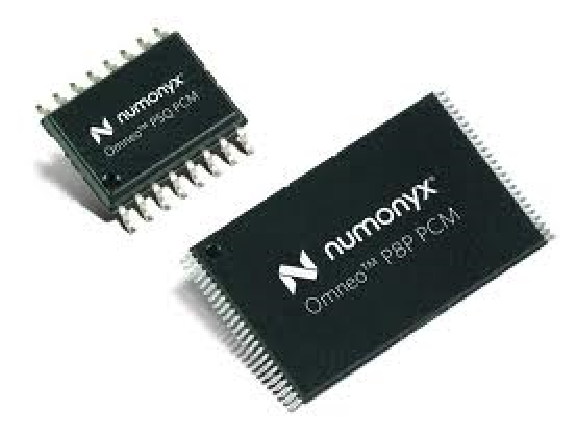
\includegraphics[angle=0, width=0.2\textwidth]{PCM_numonyx.eps}}\\
\vspace{1ex}
\textcolor{themecolor}{Numonyx} (acquisita da \textcolor{themecolor}{Micron}) ha commercializzato un dispositivo PCM di 90~nm\\
%Research center based in Agrate Brianza\\
\vspace{3ex}
{\ev Aprile 2011}\\
%\vspace{1ex}
\begin{columns}[c]
	\column{0.0\textwidth}
	\column{0.7\textwidth}
		\textcolor{themecolor}{Nokia}: telefono cellulare ``Asha'' con\\
		dispositivo PCM Micron %(NOR replacement)\\
%
	\column{0.30\textwidth}
		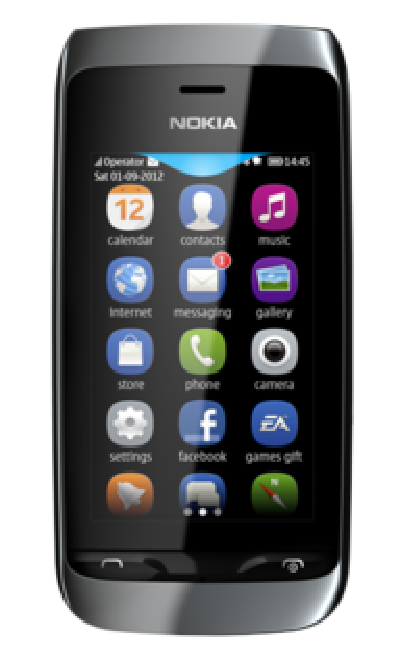
\includegraphics[angle=0, width=0.4\textwidth]{nokia.eps}
\end{columns}
%
{\ev Dicembre 2012}\\
\vspace{1ex}
\textcolor{themecolor}{Micron}: primo dispositivo a 45~nm\\ %(Agrate)\\
\end{frame}
\note{%
I dispositivi PCM sono già presenti sul mercato sin dal 2010 e nel 2011 è stato reso disponibile il primo telefono cellulare equipaggiato con un dispositivo PCM prodotto da Micron.
}


%\subsection{I nanofili e la cristallizzazione}

\begin{frame}{Nanofili nei dispositivi PCM}
 \begin{exampleblock}{Vantaggi nell'utilizzo di nanofili}
  \begin{itemize}
   \item Riduzione delle dimensioni della cella
   \item Riduzione della potenza dissipata nel processo di programmazione
   \item Effetti di confinamento del calore
  \end{itemize}
\end{exampleblock}
\note<1>{%
  Nonostante dispositivi PCM siano già stati commercializzati, sono state proposte diverse architetture per migliorarne il funzionamento e per ridurre la potenza dissipata nel processo di programmazione. Una di queste consiste nel sostituire al film di materiale attivo un nanofilo, che permette un miglior confinamento del calore e in principio consente anche una riduzione delle dimensioni della cella.
}
\end{frame}


\begin{frame}{La cristallizzazione}
\only<1-2>{%
 \begin{exampleblock}{}
 La cristallizzazione determina la velocità di \emph{switching} nei dispositivi
 \end{exampleblock}
\vspace{.5cm}
%\only<2>{%
% \begin{alertblock}{}
% La cinetica di cristallizzazione è di difficile approccio sperimentale\\[3pt]
% \end{alertblock}
%}
\visible<2>{%
 \centering
 {\bfseries Teoria della nucleazione e crescita}\\[0.5cm]
 \begin{columns}
  \begin{column}{0.5\textwidth}
   \centering
   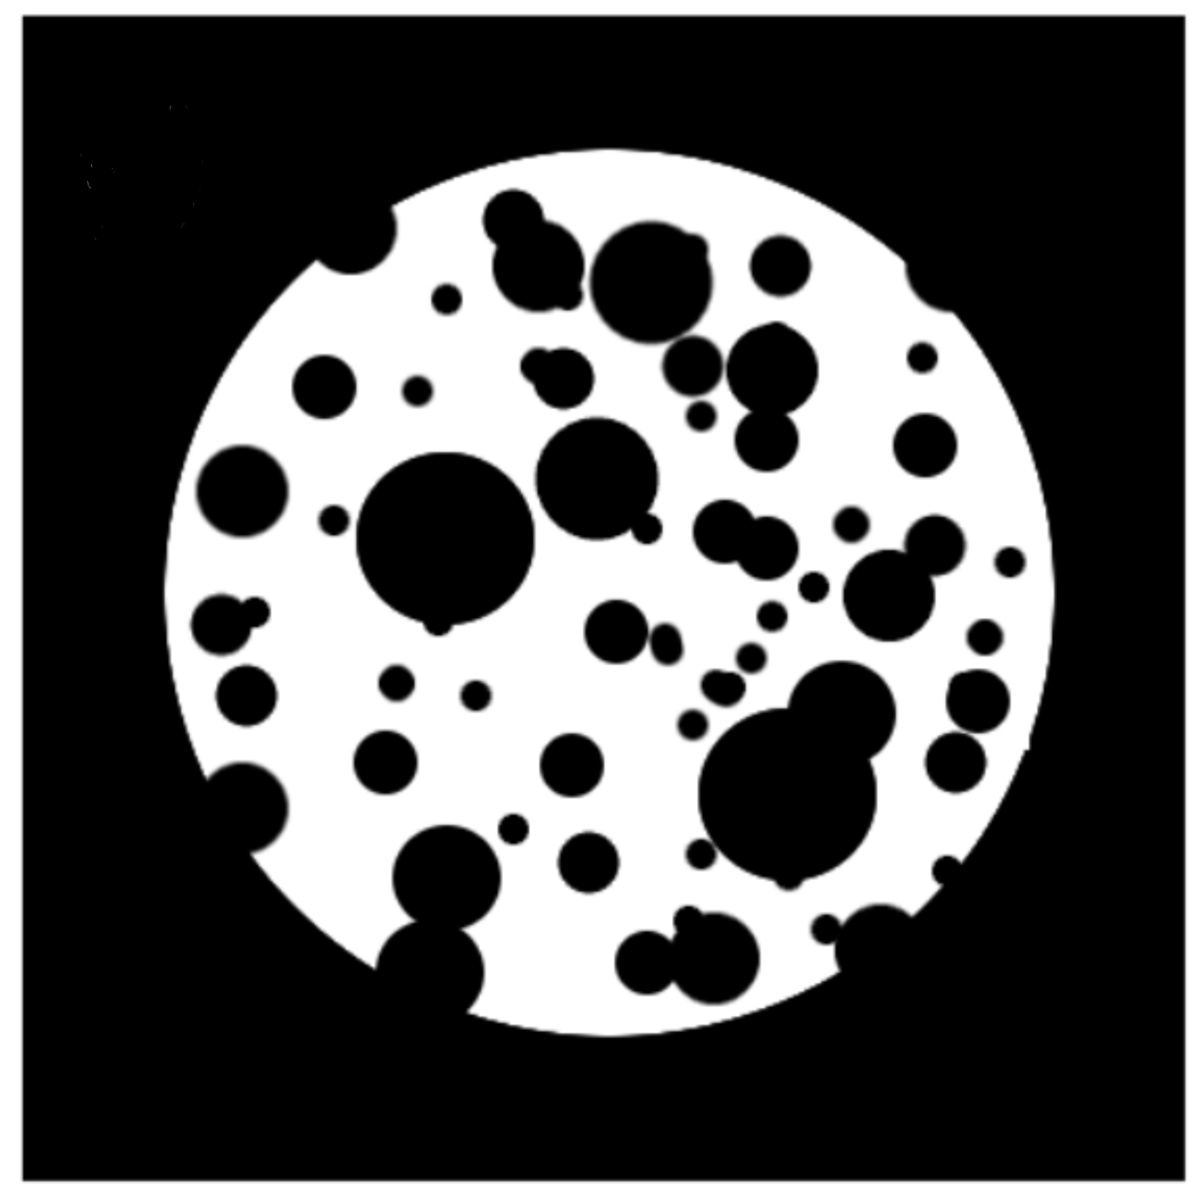
\includegraphics[width=0.3\textwidth]{N-dominated}\\[6pt]
   {\ev \emph{Nucleation--driven}}
  \end{column}
  \begin{column}{0.5\textwidth}
   \centering
   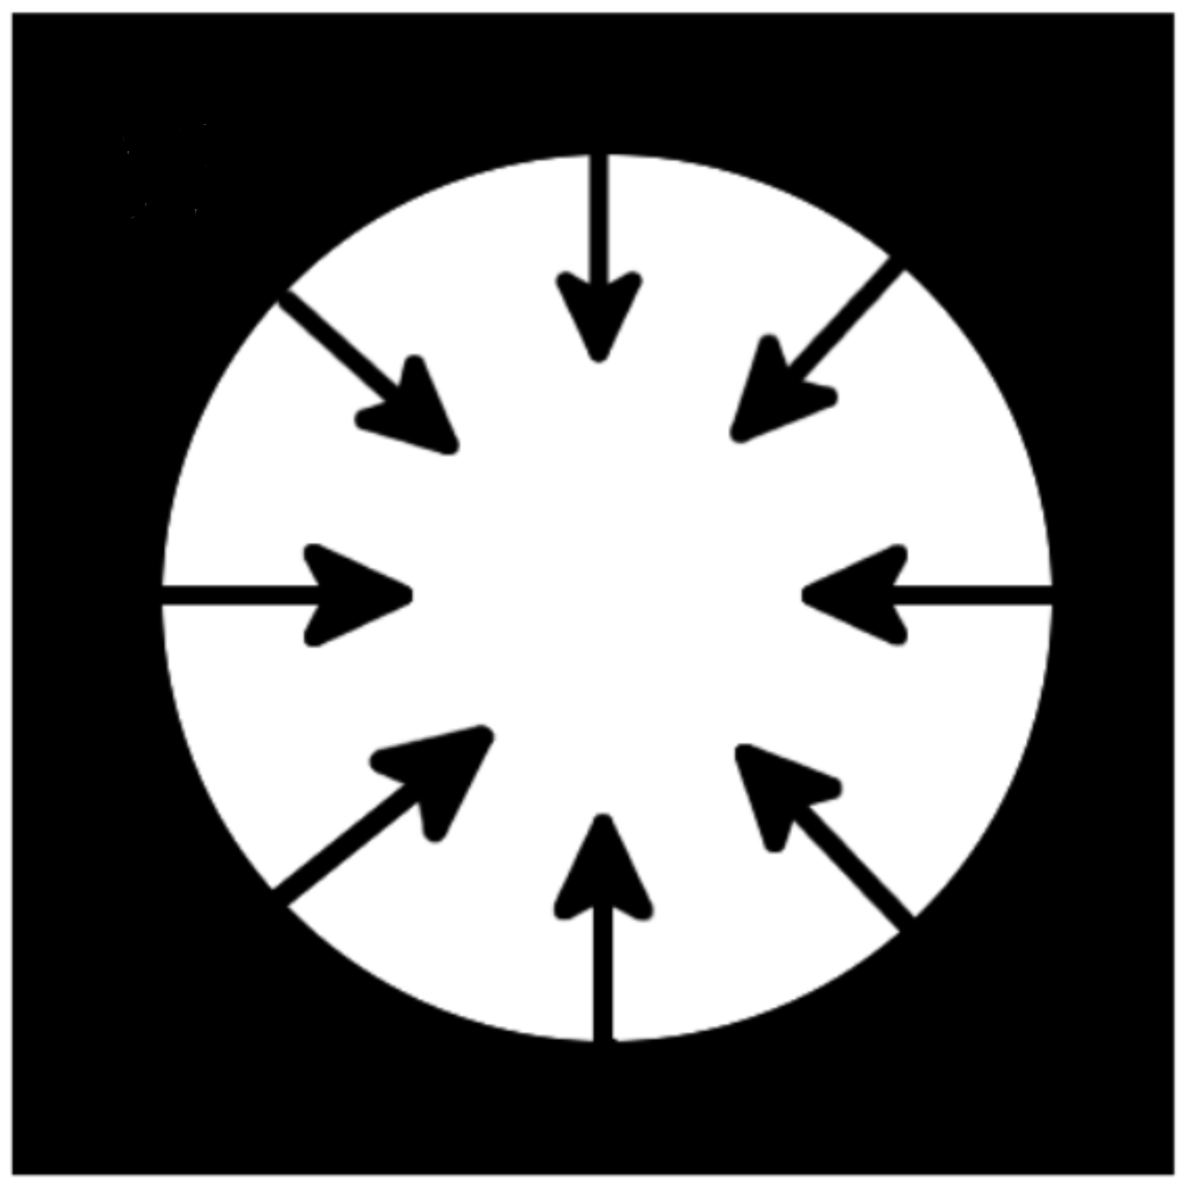
\includegraphics[width=0.3\textwidth]{G-dominated}\\[6pt]
   {\ev \emph{Growth--driven}}
  \end{column}
 \end{columns}
 }
}
\note<2>{%
 (PRIMA) Si è visto come il processo alla base del funzionamento di un dispositivo PCM sia la transizione tra la fase cristallina e quella amorfa. In particolare, il fenomeno della cristallizzazione determina la rapidità con cui è possibile cambiare lo stato di una cella di memoria.\\
 (SECONDA) Nel processo di cristallizzazione possono essere distinte due fasi: la nucleazione, ossia la formazione di un germe cristallino all'interno di una matrice disordinata, e la crescita, ossia la progressione del fronte che separa la fase cristallina da quella amorfa. Durante una cristallizzazione questi due fenomeni possono manifestare andamenti in funzione della temperatura molto diversi; è infatti possibile che uno dei due meccanismi sia dominante sull'altro, e si può distinguere un processo di cristallizzazione controllato dalla nucleazione oppure dalla crescita.
}
%\vspace{.1cm}
\only<3>{%
 \begin{alertblock}{Perché è interessante?}
  \begin{enumerate}
   \item Il meccanismo di cristallizzazione dipende dalla  dimensione della fase amorfa, dalla temperatura e dal materiale
   \item Nelle PCM la fase amorfa è portata a $T$ molto maggiori di $T\ped{glass}$ ({\bf liquido sotto--raffreddato})
   \item La cinetica di cristallizzazione può cambiare da \emph{bulk} a nanofili \\[3pt]
      $\Rightarrow\,T\ped{melt}\; \text{e}\; T\ped{glass}$ {\bf dipendono} dalle dimensioni
  \end{enumerate}
 \end{alertblock}
 }
 \note<3>{%
 (TERZA) Perciò, è interessante studiare come la cristallizzazione dipenda dalle dimensioni della fase disordinata, dalla temperatura del sistema e dal materiale. Inoltre, nei dispositivi, durante il processo di SET la fase amorfa è portata a temperature molto maggiori della temperatura di transizione vetrosa e la cristallizzazione ha luogo in quella che è chiamata ``fase liquida sotto--raffreddata''. Infine, è interessante comprendere se la cinetica di cristallizzazione subisce effetti dovuti alla dimensionalità del sistema, passando dal materiale in bulk a quello nanostrutturato.
 In questo lavoro, abbiamo studiato la cristallizzazione in nanofili costituiti dal materiale a cambiamento di fase \gete.
}

\end{frame}







\section{Nanofili di \gete}

%\subsection{\gete}

\begin{frame}{\gete: struttura cristallina}
 \begin{columns}
  \begin{column}{0.4\textwidth}
      \begin{itemize}
       \item Struttura cristallina {\ev trigonale} (fase $\alpha$) \\ Cella elementare {\ev romboedrica}
       \item Struttura cubica tipo \ce{NaCl} elongata lungo la $\langle 111 \rangle$
       \item Parametri strutturali
      %\onslide<3->{% 
       %\begin{itemize}
        %\item 
        $a=\SI{4.31}{\angstrom}$\\
        %\item 
        $\alpha=\ang{57.9}$\\
        %\item 
        $x=\num{0.2366}$ \\[3pt] Ge: $(x,\,x,\,x)$ \\[3pt] Te: $(-x,\,-x,\,-x)$
       %\end{itemize}
       %}
      \end{itemize}
  \end{column}
  \begin{column}{0.4\textwidth}
   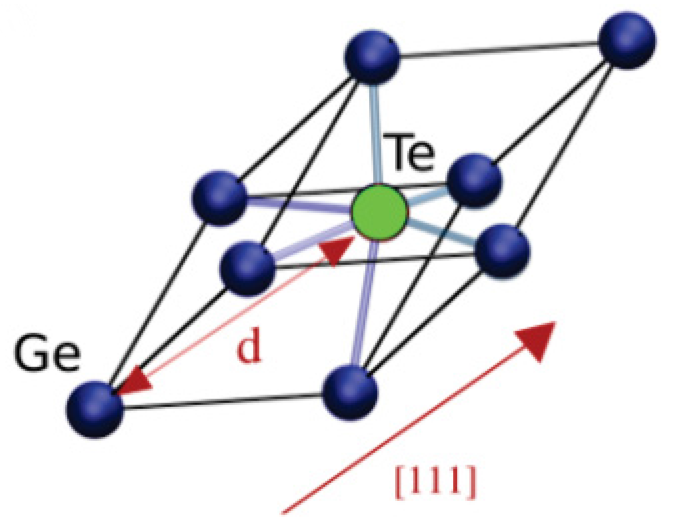
\includegraphics[width=0.7\textwidth]{GeTe-cell}\\[12pt]
   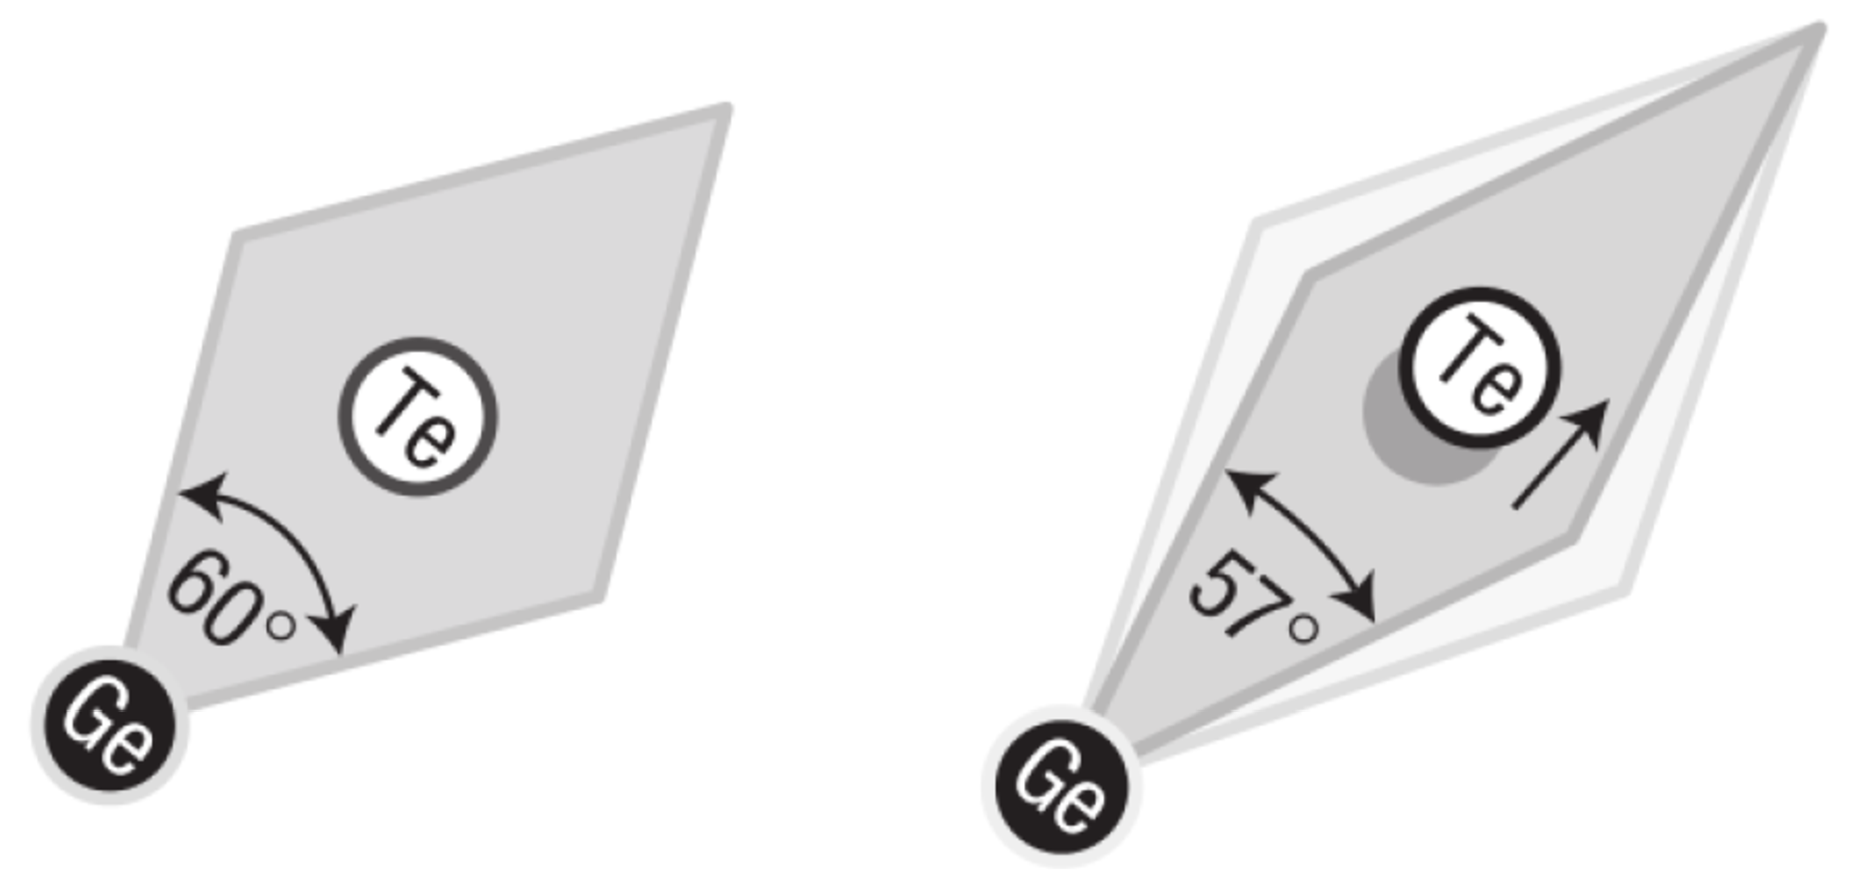
\includegraphics[width=\textwidth]{GeTe-crystal-struct}
  \end{column}

 \end{columns}

\end{frame}
\note{%
 La struttura cristallina del \gete, stabile a temperatura ambiente, è un reticolo cristallino trigonale, con una cella elementare romboedrica, mostrata in figura. Questa struttura può essere vista come la cella primitiva del reticolo cubico a facce centrate allungata lungo la direzione <111>.\\
 I parametri strutturali della struttura trigonale sono il passo reticolare $a$, l'angolo tra una coppia di vettori di base $\alpha$ e il parametro interno $x$ che assegna le posizioni nella cella elementare dei due atomi di Ge e Te.
}



%\subsection{Nanofili}

\begin{frame}{Nanofilo: il modello}
 \begin{columns}
  \begin{column}{0.5\textwidth}
    \begin{itemize}
      \item Nanofilo cresciuto lungo la {\ev direzione $[110]$}\\ (notazione esagonale)
      \item Diametro di $\sim \SI{8}{nm}$
      \item Supercella di simulazione \\ {\ev$l=\SI{84.65}{\angstrom}$} e {\ev\num{16540} atomi}
      \item PBC lungo l'asse di crescita
  \end{itemize}
  \end{column}
  \begin{column}{0.5\textwidth}
   \centering
   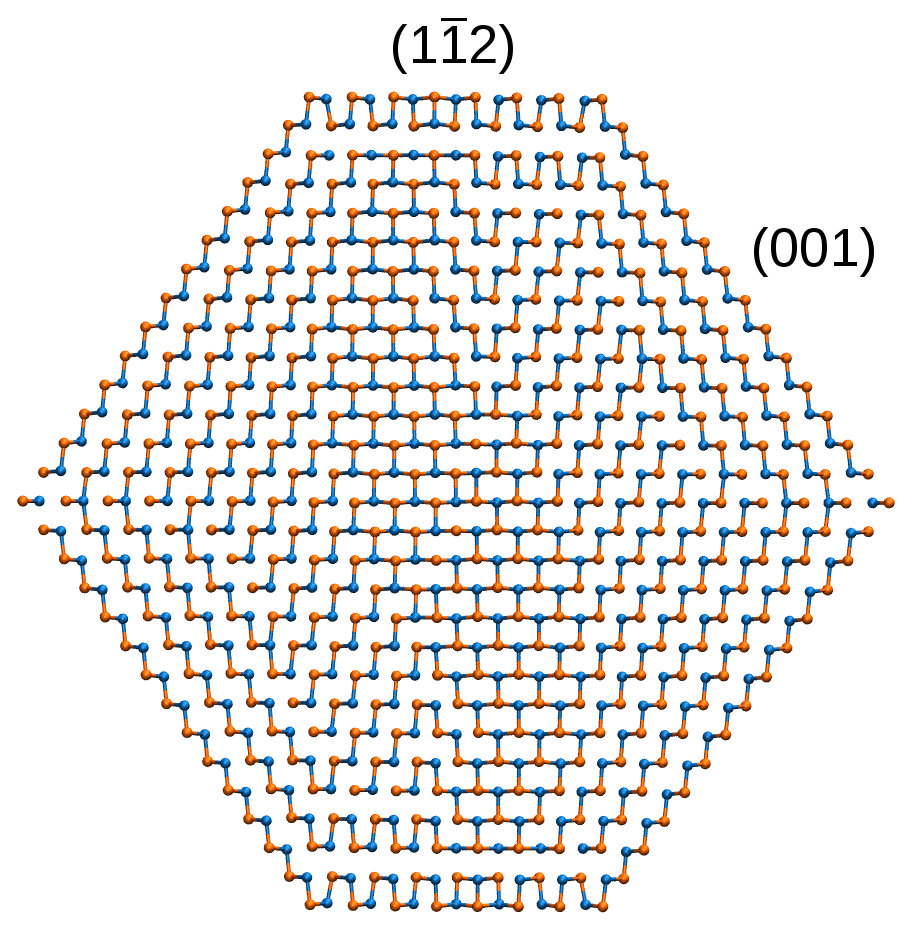
\includegraphics[width=0.35\textheight]{nw_section_OK}\\[3pt]
   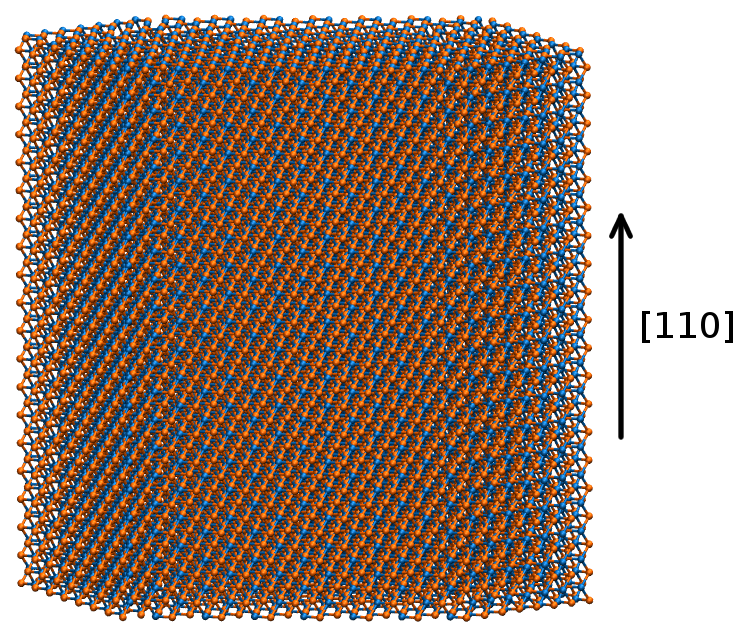
\includegraphics[width=0.35\textheight]{nw_long_OK_wDir}
  \end{column}
 \end{columns}
 \vspace{0.2cm}
 \centering
%\onslide<2->{%
 Simulazioni di {\ev dinamica molecolare} del processo di cristallizzazione% con potenziale interatomico
%}
\end{frame}
\note{%
 Il sistema considerato in questo lavoro è un nanofilo di \gete cresciuto lungo la direzione cristallografica [110], osservata in alcuni studi sperimentali, e con un diametro pari a circa 8 nm. La cella di simulazione ha una lunghezza di 84.65 angstrom e contiene 16 540 atomi.\\
 Il processo di cristallizzazione è stato studiato con simulazioni di dinamica molecolare. Poiché un numero di atomi così elevato rende inaccessibile un approccio 
}





\section{Metodi computazionali}

%\subsection{Potenziale \emph{neural networks}}
%\begin{frame}{Dinamica molecolare con potenziale \emph{neural networks}}
% MD e potenziale NN
%\end{frame}

%\subsection{Potenziale NN}

\begin{frame}{Potenziale \emph{neural networks}}
 \centering
Energia totale come somma di energie atomiche: $E_{tot} = \sum_i E_i$
\note<1>{%
The neural network potential is built by writing the total energy as 
a sum of the atomic energies which depend on the atomic local environment. 
And the local environment is described by the symmetry functions $G$ 
which depend on bond lengths and bond angles up to a certain cut-off distance 
that in our case include the third coordination shell.\\
The neural network is a scheme to assign an energy to a single atom given the 
local environment. The atomic energy is an analytic function of the atomic 
positions, so it is easy to calculate forces. 
}
\begin{flushright}
{\cit{[J.~Behler e M.~Parrinello, PRL 98, 146401 (2007)]}}
\end{flushright}
%
%\vspace{3ex}
\onslide<2->{%
  \begin{columns}[c]
    \begin{column}{0.50\textwidth}
      \begin{equation*}
	E_i = F(\{G(\vec{x})\}) 
      \end{equation*}
      \vspace{.5cm}
      \centering
      \resizebox*{0.8\textwidth}{!}{%%% TiKz picture of NN scheme
\begin{tikzpicture}
  %%Create a style for the arrows we are using
  \tikzset{normal arrow/.style={draw,-stealth',very thick,color=themecolor}}
  \tikzset{little arrow/.style={draw,-stealth',thick,color=themecolor!60!white}}
  \tikzset{node circle/.style={circle,shading=ball,ball color=themecolor,text=white}}
  \tikzstyle{layer} = [text width=4em, text centered]
  %%Create the different coordinates to place the nodes
  \path (0,0) coordinate (g1) ++(0,-2.5) coordinate (g2); %++(0,-2) coordinate (3);
  \path (g1) ++(-1.3,-.5) coordinate (x1);
  \path (g2) ++(-1.3,+.5) coordinate (x2);
  %%Use the calc library and partway modifiers to generate the second and third level points
  \path ($(g1)!.5!(g2)!2.2 cm!90:(g2)$) coordinate (y2);
  \path (y2) ++(0,2) coordinate (y1);
  \path (y2) ++(0,-2) coordinate (y3);
  \path (y2) ++(1.7,0) coordinate (e);
  %%Place nodes at each point using the foreach construct
  \foreach \in/\i/\color in {g1/1/themecolor!60,g2/2/themecolor!60}{
%    \node[draw,circle,shading=axis,top color=\color, bottom color=\color!black,text=white,shading angle=45] (n\in) at (\in) {$G_{\i}$};
    \node[node circle] (n\in) at (\in) {$G_{\i}$};
  }
  \foreach \in/\i/\color in {y1/1/themecolor!60,y2/2/themecolor!60,y3/3/themecolor!60}{
%    \node[draw,circle,shading=axis,top color=\color, bottom color=\color!black,text=white,shading angle=45] (n\in) at (\in) {$y_{\i}$} 
%         node[above of =n\in,node distance=2em]{$f_{\i}$};
    \node[node circle] (n\in) at (\in) {$y_{\i}$} node[above of =n\in,node distance=2em]{$f_{\i}$};
  }
%  \node[draw,circle,shading=axis,top color=themecolor!60, bottom color=themecolor!60!black,text=white,shading angle=45] (ne) at (e) {$\;\;E_{i}\;\;$}; 
  \node[node circle] (ne) at (e) {$\;\;E_{i}\;\;$};
  %%Place the remaining nodes separately
  \node (nx1) at (x1) {$\bm{x}_1$};
  \node (nx2) at (x2) {$\bm{x}_2$};
  %%Layer titles
  \node[layer,above of=ny2, node distance=22ex] (hl) {Hidden layer};
  \node[layer,left of=hl, node distance=2.2cm] (il) {Input layer};
  \node[layer,above of=e, node distance=22ex] (ol) {Output layer};
  %%Drawing the arrows
  \path[little arrow] (nx1) -- (ng1);
  \path[little arrow] (nx1) -- (ng2);
  \path[little arrow] (nx2) -- (ng1);
  \path[little arrow] (nx2) -- (ng2);
  \path[normal arrow] (ng1) -- node[above=.0em] {$a_{11}^{01}$} (ny1);
  \path[normal arrow] (ng1) -- node[above=.0em] {$a_{12}^{01}$} (ny2);
  \path[normal arrow] (ng1) -- node[below=-2.0em,left=1.4em] {$a_{13}^{01}$} (ny3);
  \path[normal arrow] (ng2) -- (ny1);
  \path[normal arrow] (ng2) -- (ny2);
  \path[normal arrow] (ng2) -- node[below=0.0em] {$a_{23}^{01}$} (ny3);
  \path[normal arrow] (ny1) -- node[above=0.2em] {$a_{11}^{12}$} (ne);
  \path[normal arrow] (ny2) -- node[above=0.1em] {$a_{21}^{12}$} (ne);
  \path[normal arrow] (ny3) -- node[above=0.5em] {$a_{31}^{12}$} (ne);
\end{tikzpicture}}
    \end{column}
\note<2>{%
This picture represent a simple scheme of a neural network.
The symmetry functions are obtained from the atomic positions and are the input 
values of the network. We take a linear combination of the symmetry functions with 
these weights $a$ to obtain these intermediate values $y$. Then we apply a non linear 
function $f$ with this form to the $y$s and the results are again linearly combined to 
obtain the atomic energy. The weights $a$ are the fitting parameters of the potential. 
In our case for GeTe the network has 8 thousand parameters fitted on 30 thousand 
configurations.  
}
%
\begin{column}{0.50\textwidth}
\centering
{\ev{Symmetry functions $\{G\}$}}\\
Informazioni sull'intorno atomico entro un certo raggio di \emph{cutoff} (terza \emph{shell} di coordinazione)\\[12pt]}
\onslide<3->{%
  $E_i$ è funzione analitica delle posizioni degli atomi
  \begin{equation*}
    E_i = \sum_{j=1}^3{a_{j1}^{12}\cdot f\left(\sum_{k=1}^2{G_k\cdot a_{kj}^{01}}\right)}
  \end{equation*}

}
\end{column}
\end{columns}
\end{frame}


%\subsection{Potenziale NN per il \gete}
\begin{frame}{Potenziale \emph{neural networks} per il \gete}
\only<1>{%
  \begin{itemize}
    \item $E_i$ è calcolata con il metodo \emph{neural networks}
    \item Il potenziale per il \gete è ottenuto interpolando un database di energie calcolate \emph{ab initio}
    \item \num{30000} configurazioni e $\sim\num{8000}$ parametri
  \end{itemize}
}
%
\only<2>{%
 \begin{columns}
  \begin{column}{0.5\textwidth}
  \centering
  {\footnotesize\textcolor{themecolor}{Funzioni di correlazione di coppia per \gete amorfo a \SI{300}{K}}}\\
   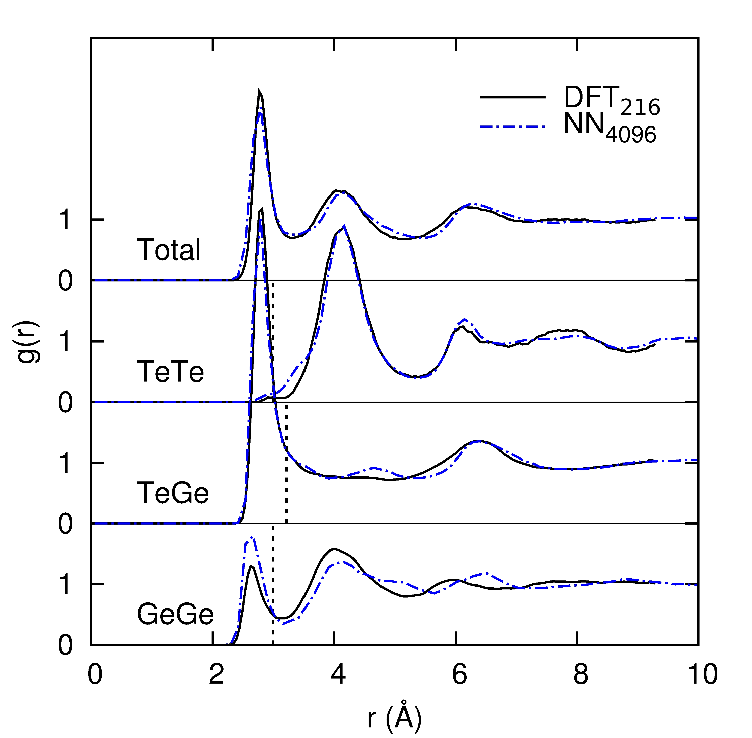
\includegraphics[width=\textwidth]{GT_grNN_DFT}\\
   %{\Large\slshape FIGURA}\\[0.2cm]   
   {\cit{[Sosso et al., PRB 85, 174103 (2012)]}}
  \end{column}
  \begin{column}{0.5\textwidth}
   \begin{itemize}
    \item Il potenziale NN descrive accuratamente le proprietà della fase liquida/amorfa del \gete
    \item Coefficiente di diffusione $D$ {\ev \SI{4.29e-5}{\square\centi\metre\per\second}}\\ (DFT~\SI{4.29e-5}{\square\centi\metre\per\second})
    \item $T\ped{m}=$ {\ev\SI{1001}{K}}\\ (exp.~\SI{998}{K})
   \end{itemize}
  \end{column}
 \end{columns}
 }
\end{frame}





\section{Risultati}

%\subsection{\gete \emph{bulk}}

\begin{frame}{Cristallizzazione in \gete \emph{bulk}}
\only<1>{%
\centering
Interfaccia tra cristallo e liquido sotto--raffreddato
  \begin{columns}
  \begin{column}{0.5\textwidth}
   \begin{itemize}
    \item Simulazioni $NVT$ per $\sim \SI{100}{ps}$
    \item Atomi cristallini identificati secondo il parametro d'ordine
      \[ \mathsmaller{q_{4m}(i) = \frac{1}{N_b (i)} \sum_{j=1}^{N_b(i)} Y_{4m}(\bm{r}_{ij})} \]
      \begin{flushleft}
       {\cit{[Steinhardt et al., PRB 28, 784 (1983)]}}
      \end{flushleft}
    \item Spessore dello \emph{slab} cristallino L\ped{cris} in funzione di t
   \end{itemize}
  \end{column}
%
  \begin{column}{0.5\textwidth}
  \centering
   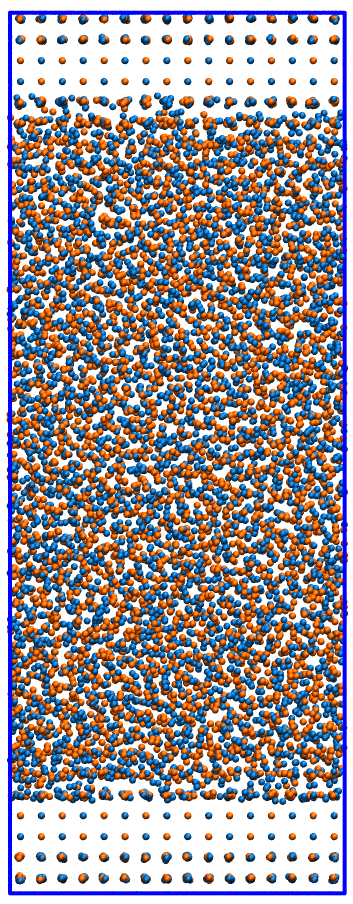
\includegraphics[scale=0.15]{m1_long_OK}\quad
   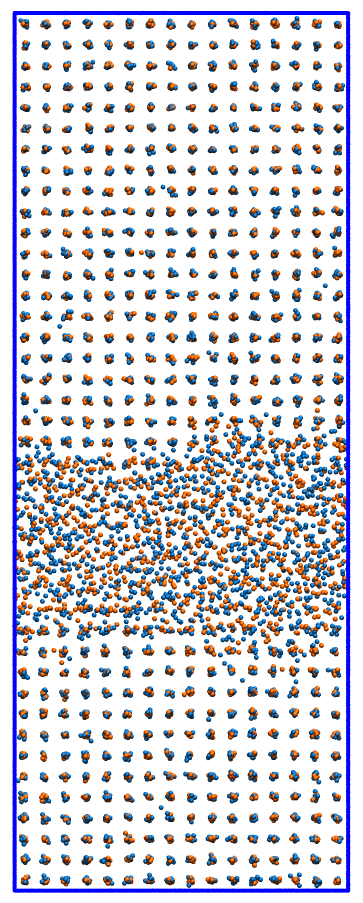
\includegraphics[scale=0.15]{m1_AfterCry}
  \end{column}
 \end{columns}
}
\only<2>{%
  \begin{columns}
   \begin{column}{0.5\textwidth}
    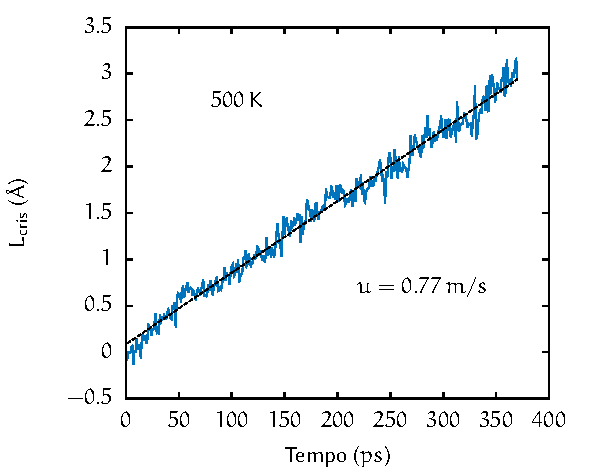
\includegraphics[width=\textwidth]{bulk_Lcr_500_OK}
   \end{column}
   \begin{column}{0.5\textwidth}
    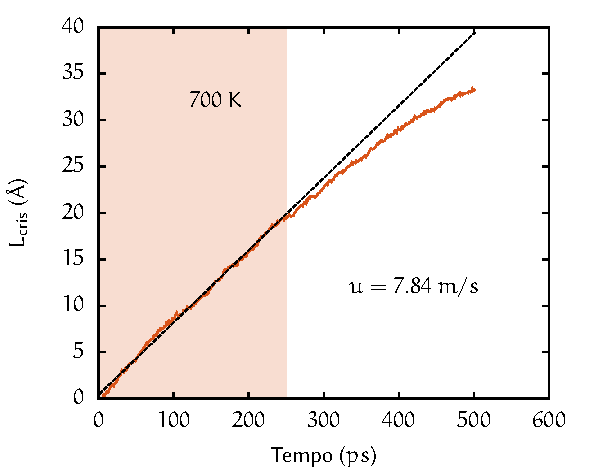
\includegraphics[width=\textwidth]{bulk_Lcr_700_OK}
   \end{column}
  \end{columns}
 \vspace{.5cm}
 \centering
 Velocità di crescita
 \[ u = \frac{dL\ped{cris}}{dt} \]
}
\end{frame}



\begin{frame}{Temperatura di fusione}
\centering
Stima della temperatura di fusione nei nanofili\\[12pt]
\begin{columns}
\begin{column}{0.4\textwidth}
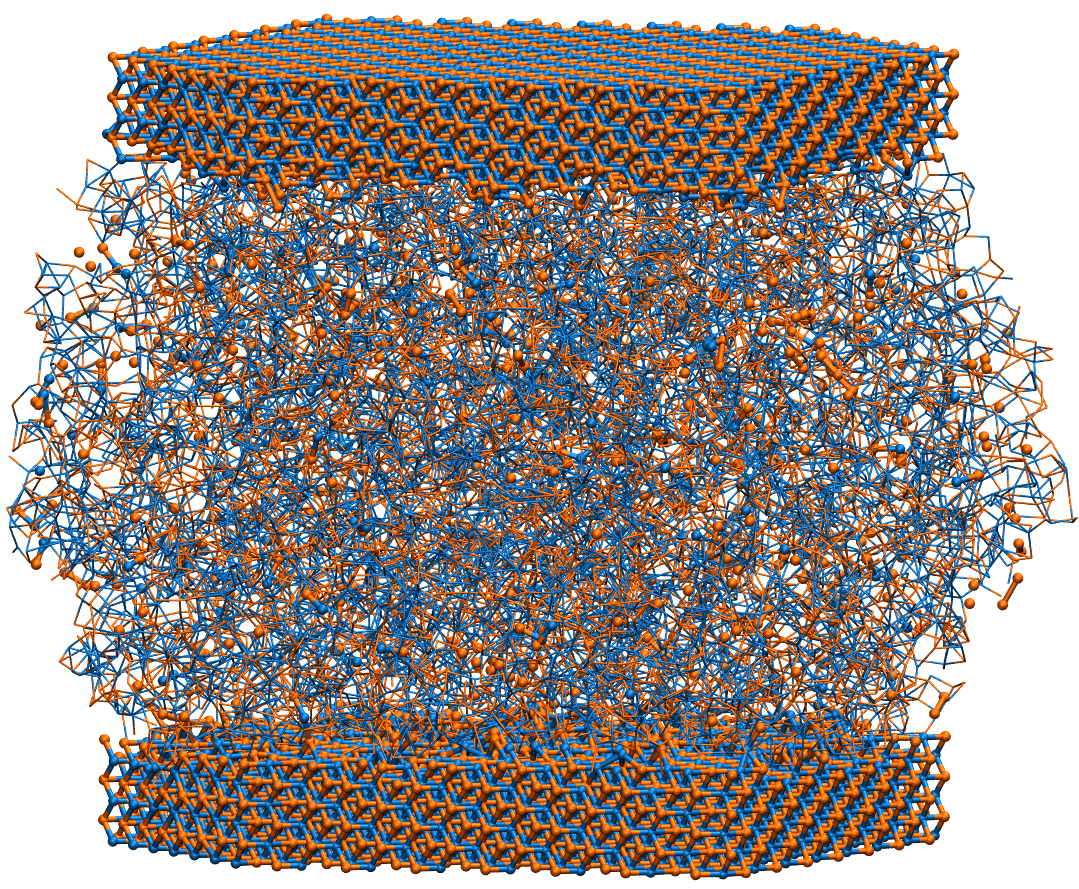
\includegraphics[width=\textwidth]{nw_superc_OK}
\end{column}
%
\begin{column}{0.6\textwidth}
%\begin{itemize}
%\item
 4 simulazioni $NVT$ a \num{800}--\num{850}--\num{900}--\SI{950}{K}%\\[3pt]
  \begin{itemize}
    \item a \SI{800}{K} {\ev cristallizzazione}
    \item a \SI{850}{K} {\ev fusione}
  \end{itemize}
%\end{itemize}
\end{column}
\end{columns}
\visible<2->{%
\begin{exampleblock}{Riduzione di T\ped{melt}}
\centering
  $\SI{800}{K} < T\ped{m}^N < \SI{850}{K}$\\[6pt]
  $T\ped{m}^B \sim \SI{1000}{K}$
\end{exampleblock}
}

\end{frame}



%\subsection{Generazione del liquido}

\begin{frame}{Generazione del liquido \emph{supercooled}}
 \begin{columns}
  \begin{column}{0.5\textwidth}
   \begin{itemize}
    \item Generato portando una parte del nanofilo a $T > T_m$ in \SI{30}{ps}
    \item Equilibrato per \SI{10}{ps} in $NVE$
    \item Raffreddato rapidamente (\SI{30}{ps}) a \num{700}--\num{600}--\SI{500}{K}
   \end{itemize}

  \end{column}
  \begin{column}{0.5\textwidth}
   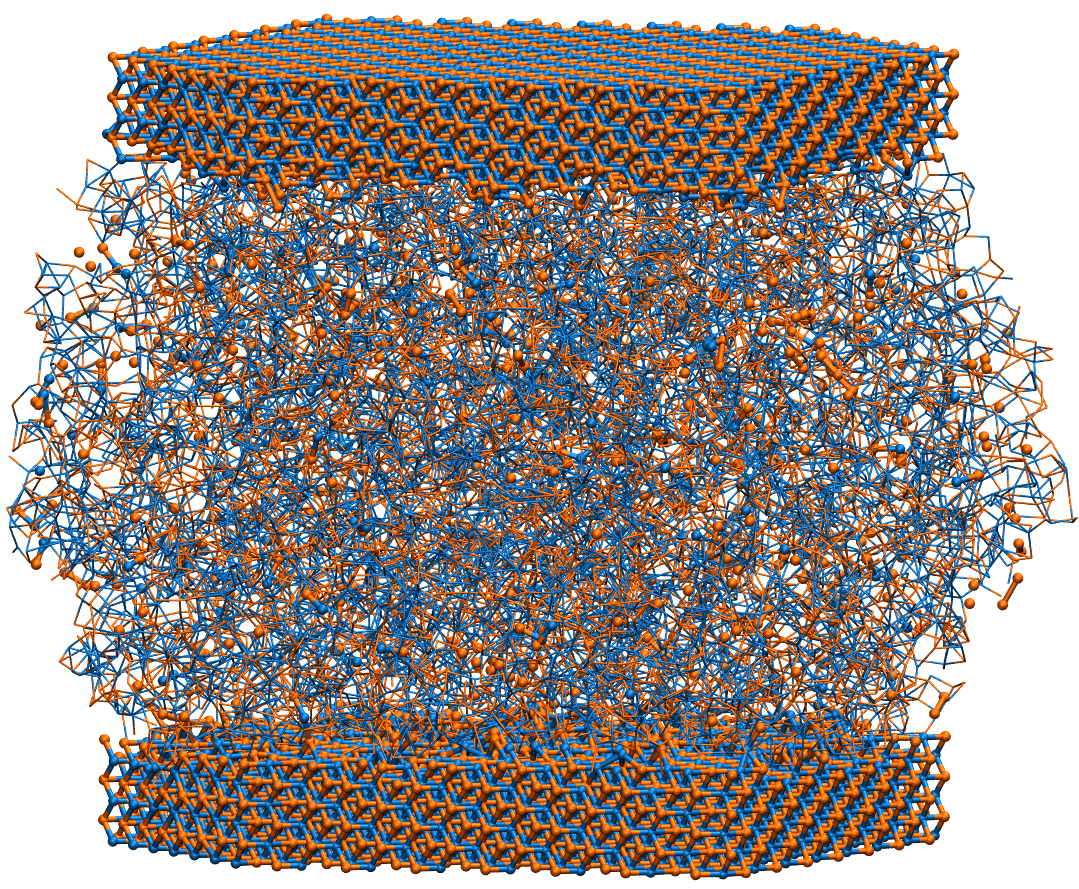
\includegraphics[width=\textwidth]{nw_superc_OK}
  \end{column}
 \end{columns}
\end{frame}


\begin{frame}{Cristallizzazione nel nanofilo}
  \begin{columns}
   \begin{column}{0.5\textwidth}
    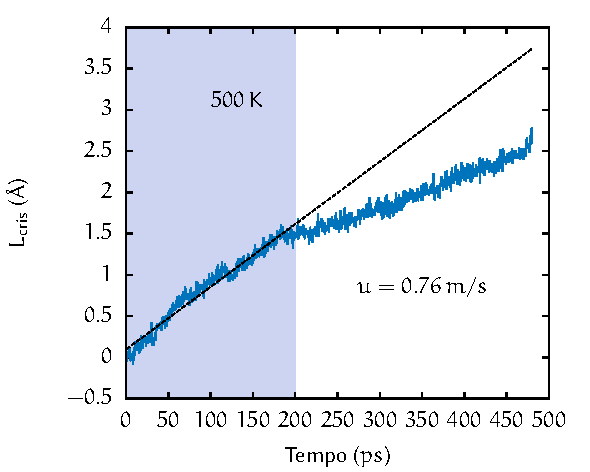
\includegraphics[width=\textwidth]{nw_Lcr_500_OK}
   \end{column}
   \begin{column}{0.5\textwidth}
    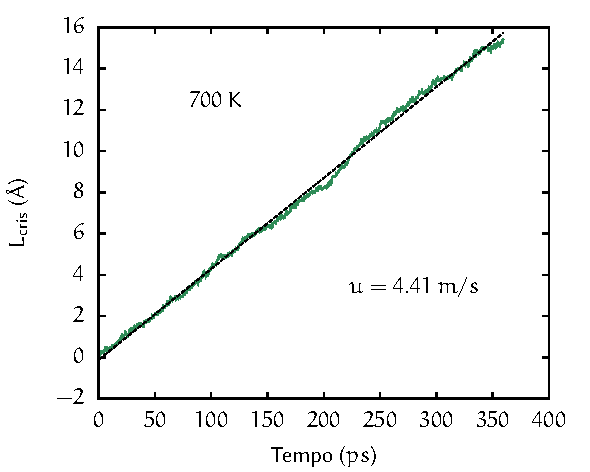
\includegraphics[width=\textwidth]{nw_Lcr_700_OK}
   \end{column}
  \end{columns}
  \begin{table}[h]
   \resizebox*{0.3\textwidth}{!}{%
    \begin{tabular}{cSS}
     	\toprule
     	\rowcolor{themecolor!20!white}
	T (\si{K}) & \multicolumn{2}{S}{ {u (\si{\metre\per\second})} } \\
	\cmidrule{2-3}
		& {\small Nanofilo} & {\small Bulk} \\
	\midrule
	\num{500} & 0.76 & 0.77 \\
	\num{700} & 4.41 & 7.84 \\
	\bottomrule
    \end{tabular}}
  \end{table}

\end{frame}




\begin{frame}{Velocità di cristallizzazione}
 Velocità di crescita secondo la \emph{teoria classica della nucleazione}
 %\centering
  \begin{equation*}
    u(T)= \frac{6D}{\lambda} \left[ 1- e^{ \left( -\Delta\mu/k_B T\right) } \right]
  \end{equation*}
  \begin{center}
  \begin{description}
   \item [$D$] coefficiente di auto--diffusione
   \item [$\lambda$] distanza interatomica media ($\sim \SI{3}{\angstrom}$)
   \item [$\Delta\mu$] differenza di potenziale chimico tra cristallo e liquido
  \end{description}  
  \end{center}
\end{frame}


\begin{frame}{Coefficiente di auto--diffusione}
 \begin{columns}
  \begin{column}{0.5\textwidth}
   Calcolato con la \emph{relazione di Einstein}
   \begin{equation*}
    \frac{\partial\langle r^2(t)\rangle}{\partial t}=6D
   \end{equation*}
   Energia di attivazione
   \begin{equation*}
    \begin{split}
        &E_a = \SI{0.314}{eV}\\
	&E_a\ap{bulk} = \SI{0.4}{eV}
    \end{split}
   \end{equation*}
  \end{column}
  \begin{column}{0.5\textwidth}
  \centering
   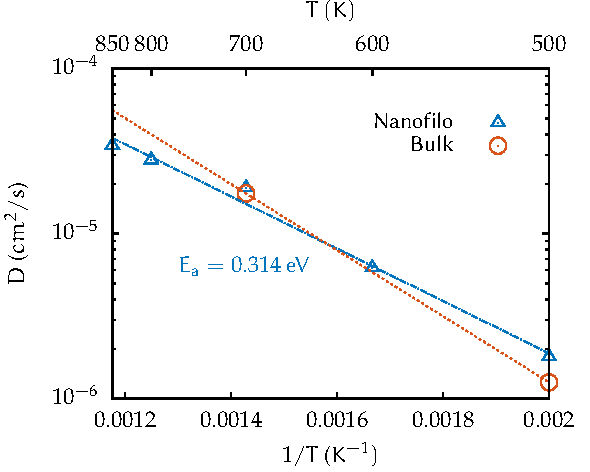
\includegraphics[scale=0.6]{D_vs_T}
   \begin{table}[h]
   \begin{center}
   \resizebox{0.6\textwidth}{!}{%
    \begin{tabular}{ccc}
     	\toprule
     	\rowcolor{themecolor!20!white}
	T (\si{K}) & \multicolumn{2}{c}{D (\SI{e-6}{\square\centi\metre\per\second})} \\
		& {\small Nanofilo} & {\small Bulk} \\
	\midrule
	\num{500} & \num{1.78} & \num{1.25} \\
	\num{700} & \num{18.9} & \num{17.5} \\
	\bottomrule
    \end{tabular}}
    \end{center}
  \end{table}
  \end{column}


 \end{columns}

\end{frame}


\begin{frame}{Differenza di potenziale chimico}
 Differenza di potenziale chimico $\Delta\mu$ tra cristallo e liquido\\[3pt]
 Formula di {\ev Thompson--Spaepen}
 \[ \Delta\mu = T_m\Delta S_m \frac{(T_m-T)\,2T}{(T_m+T)\,T_m} \]
 \begin{description}
 	\item [$T_m\Delta S_m$] calore latente di fusione
 	\item [$\Delta S_m$ (bulk)] calcolato da simulazioni NN--MD\\ pari \textcolor{themecolor}{\SI{0.186}{meV/\text{atomo}}}
 \end{description}
 
\end{frame}


\begin{frame}{Velocità di cristallizzazione}{Confronto tra nanofilo e bulk}
\only<1-2>{%
 Abbiamo osservato una {\ev diminuzione} della velocità di crescita\\[6pt]
 Supponiamo uguale il valore di $\Delta S_m$ per nanofilo e bulk
 \begin{equation*}
  \begin{split}
   u\ped{N} &= \frac{6D\ped{N}}{\lambda} \left( 1- e^{-\Delta\mu\ped{N}/k_B T} \right) \\[6pt]
   u\ped{B} &= \frac{6D\ped{B}}{\lambda} \left( 1- e^{-\Delta\mu\ped{B}/k_B T} \right)
  \end{split}
 \end{equation*}
\onslide<2>{%
 \begin{columns}[b]
  \begin{column}{0.5\textwidth}
   \begin{displaymath}
      \frac{u\ped{B}}{u\ped{N}}(\num{700}\,K) \approx \textcolor{themecolor}{\num{1.61}}
   \end{displaymath}
  \end{column}
  \begin{column}{0.5\textwidth}
   \begin{displaymath}
    \text{Da simulazioni MD} \approx \textcolor{themecolor}{\num{1.78}}
   \end{displaymath}
  \end{column}
 \end{columns}
 }
}
\only<3>{%
 \centering
 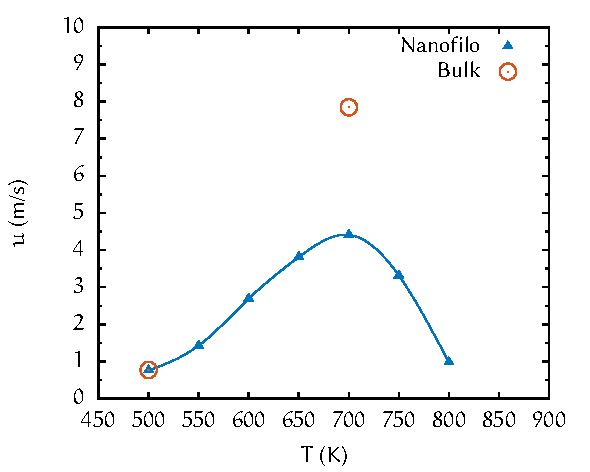
\includegraphics[scale=0.7]{u_vs_T_OnlyMine}
}


\end{frame}


\section{Conclusioni}

\begin{frame}{Conclusioni}
 \begin{itemize}
 	\item Cinetica di cristallizzazione in nanofili di \gete
 	\item Riduzione di $T_m$ da $\SI{1001}{K}$ a $\approx\SI{830}{K}$
 	\item Riduzione della velocità di cristallizzazione al più di un fattore 2, ben descritta dall'espressione classica (CNT) per la velocità di crescita
 	\item Cinetica di cristallizzazione compatibile ad utilizzo di nanofili ultra--scalati nelle celle PCM
 \end{itemize}
\centering
\vspace{0.5cm}
\onslide<2->{Progetto Europeo {\ev FP7--Synapse}}

	
\end{frame}
\note{In questo lavoro di tesi abbiamo studiato la cinetica di cristallizzazione in nanofili di gete, osservando una riduzione della temperatura di fusione da 1000 kelvin del gete bulk a circa 830 kelvin nei nanofili. Questa riduzione è responsabile della minore velocità di cristallizzazione osservata nei nanofili, che risulta essere al più un fattore 2 inferiore alla velocità calcolata nel bulk. Inoltre, l'andamento della velocità di crescita in funzione della temperatura è ben descritto dall'espressione classica.
Possiamo perciò concludere che i risultati osservati suggeriscono che nanofili ultra--scalati fino a 8 nm di diametro possano essere efficacemente impiegati nelle celle PCM. 
}



%%% BACKUP SLIDES
\appendix

\begin{frame}{Parametro d'ordine}
\only<1>{%
 \begin{equation*}
  \begin{split}
   \bar{Q}_4(i) &= \frac{1}{N_b(i)}\sum_{j=1}^{N_b(i)}%
  	\frac{\sum_{m=-4}^4 \bar{q}_{4m}(i)\, \bar{q}_{4m}^{\text{*}}(j) }{\left(  \sum_{m=-4}^4 \lvert \bar{q}_{4m}(i)\rvert^2 \right) \left(  \sum_{m=-4}^4 \lvert \bar{q}_{4m}(j)\rvert^2 \right)} \\
  	\bar{q}_{4m}(i) &= \frac{1}{\widehat{N}_{b}(i)} \sum_{k=0}^{\widehat{N}_{b}(i)} q_{4m}(k) \\
  	q_{4m}(i) &= \frac{1}{N_b (i)} \sum_{j=1}^{N_b(i)} Y_{4m}(\bm{r}_{ij})
  \end{split}
 \end{equation*}
}
\only<2>{%
 \begin{alertblock}{Criterio su $\bar{Q}_4$}
	Un atomo appartiene alla fase cristallina se $\bar{Q}_4 > 0.9$
 \end{alertblock}
	\vspace{0.5cm}
\begin{columns}
	\begin{column}{0.6\textwidth}
	%\begin{center}
		\centering
		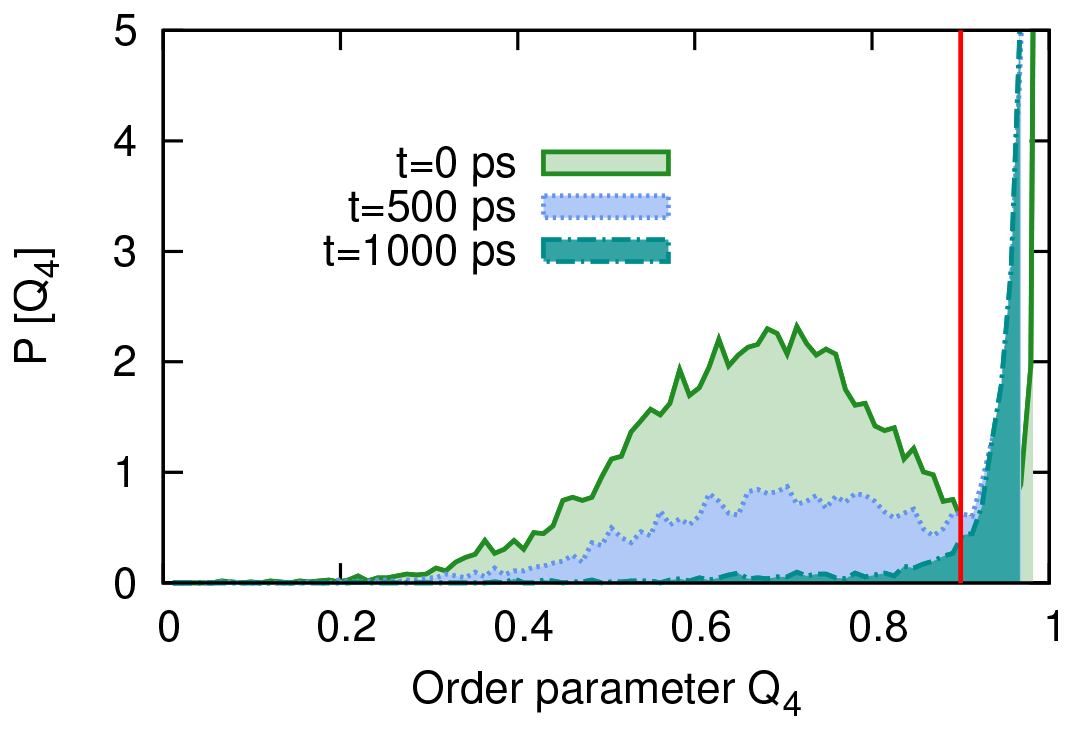
\includegraphics[scale=0.6]{Q4_dist}
	%\end{center}
	\end{column}
	\begin{column}{0.4\textwidth}
		\centering
		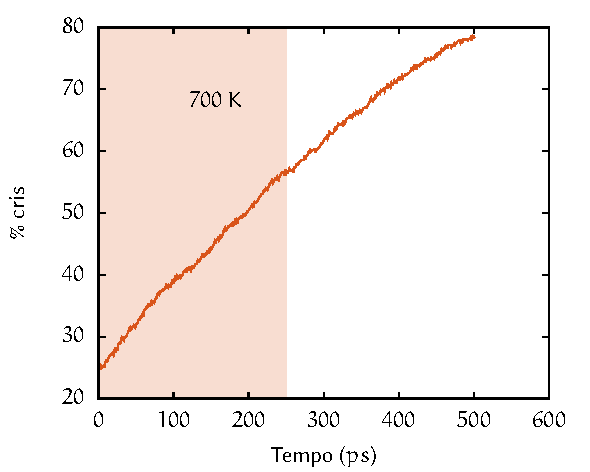
\includegraphics[scale=0.4]{Cry_frac_700}
	\end{column}
\end{columns}
}

\end{frame}

\begin{frame}{Velocità di crescita}{Calcolo di L\ped{cris}}
 La velocità di crescita è estratta da $\frac{dL\ped{cris}}{dt}$ nella regione lineare.
 \begin{equation*}
 	L\ped{cris}= N\ped{cris} \frac{d\ped{hkl}}{2 N\ped{surf}}	
 \end{equation*}
 \begin{description}
 	\item [$N\ped{cris}$] numero di atomi cristallini appartenenti allo \emph{slab} al tempo $t$
 	\item [$d\ped{hkl}$] distanza interplanare dei piani cristallini dello \emph{slab}
 	\item [$N\ped{surf}$] numero di atomi nella superficie cristallina ideale
 \end{description}	
\end{frame}



%\begin{frame}{Coefficiente di auto--diffusione}{Calcolo}
% MSD e fit lineare.
%\end{frame}

\begin{frame}{Cristallizzazione}{Confronto tra nanofilo e bulk}
\begin{center}
 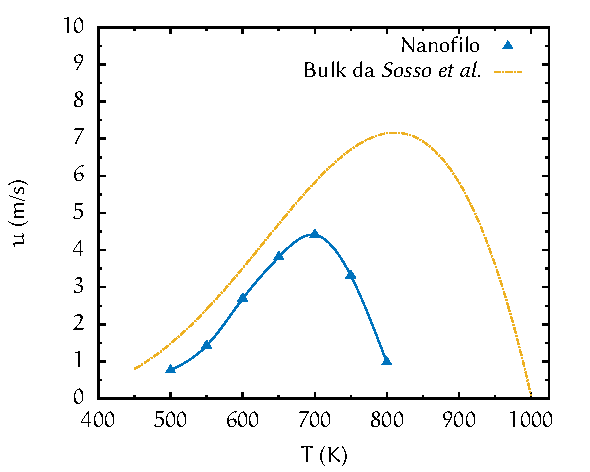
\includegraphics[scale=0.7]{u_vs_T_withSosso}\\[0.2cm]
 {\cit{[Sosso et al., J. Phys. Chem. Lett. 4, 4241 (2013)]}}
\end{center}
\end{frame}





\end{document}


